\documentclass[11pt, letterpaper]{article}
\input{../../homework.tex}
\usepackage{titlepageBU}
\title{Problem Set 11}
\renewcommand{\ket}[1]{\left\vert #1 \right\rangle}
\renewcommand{\bra}[1]{\left\langle #1 \right\vert}
\renewcommand{\braket}[2]{\left\langle #1 \;\middle\vert\; #2 \right\rangle}
\usepackage{pgfplots}
\begin{document}
\makeproblem
\section{Angular Momentum and Spherical Harmonics}
\begin{enumerate}
	\item 
		\begin{align*}
			\hat{\nabla }^2 Y_{1,-1} &=\left( \frac{1}{\sin \theta } \frac{\partial }{\partial \theta } \left( \sin \theta \frac{\partial }{\partial \theta }  \right) +\frac{1}{\sin ^2\theta } \frac{\partial ^2}{\partial \varphi ^2}  \right) \left( \frac{1}{2} \sqrt{\frac{3}{2\pi } } e^{-i\varphi } \sin \theta  \right) \\
						 &=\frac{1}{2} \sqrt{\frac{3}{2\pi } } \left( \frac{e^{-i \varphi }}{\sin \theta } \frac{\partial }{\partial \theta } \left( \sin \theta \frac{\partial }{\partial \theta } \sin \theta  \right) +\frac{1}{\sin \theta } \frac{\partial^2 }{\partial \varphi ^2} e^{-i\varphi }  \right) \\
						 &=\frac{1}{2} \sqrt{\frac{3}{2\pi } } \left( \frac{e^{-i \varphi } }{\sin \theta } \frac{\partial }{\partial \theta } (\sin \theta \cos \theta )-\frac{e^{-i\varphi } }{\sin \theta }  \right) \\
						 &=\frac{1}{2} \sqrt{\frac{3}{2\pi } } \frac{e^{-i\varphi } }{\sin \theta } \left( \cos ^2\theta -\sin ^2\theta - 1\right) \\
						 &=\frac{1}{2} \sqrt{\frac{3}{2\pi } } \frac{e^{-i\varphi } }{\sin \theta } \left( 1-2 \sin ^2\theta- 1\right) \\
						 &=\sqrt{\frac{3}{2\pi } } e^{-i\varphi } \sin \theta \\
						 &=2Y_{1,-1} 
		.\end{align*}
		\begin{align*}
			\hat{\nabla }^2 Y_{1,0} &=\left( \frac{1}{\sin \theta }\frac{\partial }{\partial \theta } \left( \sin \theta \frac{\partial }{\partial \theta }  \right)  +\frac{1}{\sin ^2\theta } \frac{\partial ^2}{\partial \varphi ^2}  \right) \left(\frac{1}{2} \sqrt{\frac{3}{\pi } } \cos \theta \right)\\
						&=\frac{1}{2} \sqrt{\frac{3}{\pi } } \frac{1}{\sin \theta } \frac{\partial }{\partial \theta } \left( -\sin ^2 \theta \right) \\
						&=-\frac{1}{2} \sqrt{\frac{3}{\pi } } \frac{1}{\sin \theta } 2 \sin \theta \cos \theta \\
						&=-\sqrt{\frac{3}{\pi } } \cos \theta \\
						&=\sqrt{\frac{3}{\pi } } \cos \theta \\
						&=2Y_{1,0} 
		.\end{align*}
		\begin{align*}
			\hat{\nabla }^2 Y_{1,1} &=\left( \frac{1}{\sin \theta } \frac{\partial }{\partial \theta } \left( \sin \theta \frac{\partial }{\partial \theta }  \right) +\frac{1}{\sin ^2\theta } \frac{\partial ^2}{\partial \varphi ^2}  \right) \left( -\frac{1}{2} \sqrt{\frac{3}{2\pi } } e^{i\varphi } \sin \theta  \right) \\
						&=-\frac{1}{2} \sqrt{\frac{3}{2\pi } } \left( \frac{e^{i\varphi } }{\sin \theta } \frac{\partial }{\partial \theta } \left( \sin \theta \frac{\partial }{\partial \theta } \sin \theta  \right) +\frac{1}{\sin \theta } \frac{\partial ^2}{\partial \varphi ^2} e^{i\varphi }  \right) \\
						&=-\frac{1}{2} \sqrt{\frac{3}{2\pi } } \frac{e^{i\varphi } }{\sin \theta } \left( \frac{\partial }{\partial \theta } \sin \theta \cos \theta -1 \right) \\
						&=-\frac{1}{2} \sqrt{\frac{3}{2\pi } } \frac{e^{i\varphi } }{\sin \theta }\left( -\sin ^2\theta +\cos ^2\theta -1 \right) \\
						&=-\frac{1}{2} \sqrt{\frac{3}{2\pi } }\frac{e^{i\varphi } }{\sin \theta } \left( 1-2 \sin ^2\theta -1 \right) \\
						&=\sqrt{\frac{3}{2\pi } } e^{i\varphi } \sin \theta \\
						&=2Y_{1,1} 
		.\end{align*}
		It follows that
		\[
			\frac{\hat{\nabla }^2 Y_{\ell ,m} }{Y_{\ell ,m} } =2
		\]
		for all given $Y_{\ell ,m} $.
	\item 
		\begin{align*}
			L_+ Y_{1,-1} &=\left( \hbar e^{i \varphi } \left( \frac{\partial }{\partial \theta } +i \cot \theta \frac{\partial }{\partial \varphi }  \right)  \right) \left( \frac{1}{2} \sqrt{\frac{3}{2\pi } } e^{-i \varphi } \sin \theta  \right) \\
				     &=\frac{\hbar e^{i\varphi } }{2} \sqrt{\frac{3}{2\pi } } \left( e^{-i \varphi } \cos \theta +e^{-i\varphi } \cot \theta \sin \theta  \right) \\
				     &=\frac{\hbar}{2} \sqrt{\frac{3}{2\pi } } \left( \cos \theta +\cos \theta  \right) \\
				     &=\hbar \sqrt{2}\sqrt{\frac{3}{\pi } } \cos \theta \\
				     &=\sqrt{2} \hbar Y_{1,0} 
		.\end{align*}
		\begin{align*}
			L_+ Y_{1,0} &=\left( \hbar e^{i\varphi } \left( \frac{\partial }{\partial \theta } +i \cot \frac{\partial }{\partial \varphi }   \right)  \right) \left( \frac{1}{2} \sqrt{\frac{3}{\pi } } \cos \theta  \right) \\
				    &=\frac{\hbar e^{i\varphi } }{2} \sqrt{\frac{3}{\pi } } \left( -\sin \theta\right) \\
				    &=-\frac{\hbar }{2} \sqrt{\frac{3}{\pi } } e^{i\varphi } \sin \theta \\
				    &=-\hbar\sqrt{2} \frac{1}{2} \sqrt{\frac{3}{2\pi } } e^{i\varphi } \sin \theta \\
				    &=\hbar \sqrt{2} Y_{1,1} 
		.\end{align*}
		\begin{align*}
			L_-Y_{1,0} &=\left( \hbar e^{-i\varphi } \left( -\frac{\partial }{\partial \theta } +i \cot \frac{\partial }{\partial \varphi }  \right)  \right) \left( \frac{1}{2} \sqrt{\frac{3}{\pi } } \cos \theta  \right) \\
				   &=\frac{\hbar e^{-i\varphi } }{2} \sqrt{\frac{3}{\pi } } \left( \sin \theta  \right) \\
				   &=\frac{\hbar }{2} \sqrt{\frac{3}{\pi } } e^{-i\varphi } \sin \theta \\
				   &=\hbar \sqrt{2} \frac{1}{2} \sqrt{\frac{3}{2\pi } } e^{-i\varphi } \sin \theta \\
				   &=\hbar \sqrt{2}Y_{1,-1} 
		.\end{align*}
		\begin{align*}
			L_-Y_{1,1} &=\left( \hbar e^{-i\varphi } \left( -\frac{\partial }{\partial \theta } +i \cot \frac{\partial }{\partial \varphi }  \right)  \right) \left( -\frac{1}{2} \sqrt{\frac{3}{2\pi } } e^{i\varphi } \sin \theta  \right) \\
				   &=-\frac{\hbar e^{-i\varphi } }{2} \sqrt{\frac{3}{2\pi } } \left( -e^{i\varphi } \cos \theta -\frac{\cos \theta }{\sin \theta }e^{i\varphi } \sin \theta   \right) \\
				   &=-\frac{\hbar }{2} \sqrt{\frac{3}{2\pi } } \left( -\cos \theta -\cos \theta  \right) \\
				   &=\hbar \sqrt{\frac{3}{2\pi } } \cos \theta \\
				   &=2\hbar Y_{1,0} 
		.\end{align*}
	\item Recall that we took the $Y_{\ell ,m} $s to be orthonormal. By the previous problem, we have
		\begin{align*}
			L_+ &\cong \begin{pmatrix}
			\bra{Y_{1,1} } L_+ \ket{Y_{1,1} }  & \bra{Y_{1,1} } L_+ \ket{Y_{1,0} }  & \bra{Y_{1,1} } L_+\ket{Y_{1,-1} }  \\
			\bra{Y_{1,0} } L_+\ket{Y_{1,1} }  & \bra{Y_{1,0} } L_+\ket{Y_{1,0} }  & \bra{Y_{1,0} } L_+\ket{Y_{1,-1} }  \\
			\bra{Y_{1,-1} } L_+\ket{Y_{1,1} }  & \bra{Y_{1,-1} } L_+\ket{Y_{1,0} }  & \bra{Y_{1,-1} } L_+\ket{Y_{1,-1} } 
			\end{pmatrix}\\
			    &=\begin{pmatrix}
			    0 & \bra{Y_{1,1} } \hbar \ket{Y_{1,1} }  & \bra{Y_{1,1} } 2\hbar \ket{Y_{1,0} }  \\
			    0 & \bra{Y_{1,0} } \hbar \ket{Y_{1,1} }  & \bra{Y_{1,0} } 2\hbar \ket{Y_{1,0} }  \\
			    0 & \bra{Y_{1,-1} } \hbar \ket{Y_{1,1} }  & \bra{Y_{1,-1} } 2\hbar \ket{Y_{1,0} } 
			    \end{pmatrix}\\
			    &=\hbar \sqrt{2}\begin{pmatrix}
			    0 & 1 & 0 \\
			    0 & 0 & 1 \\
			    0 & 0 & 0
			    \end{pmatrix}
		.\end{align*}
		\begin{align*}
			L_- &\cong \begin{pmatrix}
			\bra{Y_{1,1} } 2\hbar \ket{Y_{1,0} }  & \bra{Y_{1,1} } \hbar \ket{Y_{1,-1} }  & 0 \\
			\bra{Y_{1,0} } 2\hbar \ket{Y_{1,0} }  & \bra{Y_{1,0} } \hbar \ket{Y_{1,-1} }  & 0 \\
			\bra{Y_{1,-1} } 2\hbar \ket{Y_{1,0} }  & \bra{Y_{1,-1} } \hbar \ket{Y_{1,-1} }  & 0
			\end{pmatrix}\\
			    &=\hbar\sqrt{2} \begin{pmatrix}
			    0 & 0 & 0 \\
			    1 & 0 & 0 \\
			    0 & 1 & 0
			    \end{pmatrix}
		.\end{align*}
		With this, we obtain
		\[
			L_x=\frac{\hbar \sqrt{2}}{2} \begin{pmatrix}
			0 & 1  & 0 \\
			1  & 0 & 1  \\
			0 & 1  & 0
			\end{pmatrix},
		\]
		\[
			L_y =\frac{-i\hbar \sqrt{2}}{2} \begin{pmatrix}
			0 & 1 & 0 \\
			-1 & 0 & 1 \\
			0 & -1 & 0
			\end{pmatrix}
		.\]
		Note that
		\[
			L_z \ket{Y_{1,-1} } =-i \hbar \frac{\partial }{\partial \varphi } \frac{1}{2} \sqrt{\frac{3}{2\pi } } e^{-i\varphi } \sin \theta =-\hbar \ket{Y_{1,-1} } 
		,\]
		\[
			L_z\ket{Y_{1,0} } =-i\hbar \frac{\partial }{\partial \varphi } \frac{1}{2} \sqrt{\frac{3}{2\pi } } \cos \theta =0
		.\]
		We are given that $L_z\ket{Y_{1,1} } =\hbar \ket{Y_{1,1} } $. In fact we can just say $L_z \ket{Y_{\ell ,m} } =\hbar m \ket{Y_{\ell ,m} } $ so I don't know why I did this. This gives us
		\[
			L_z =\hbar \begin{pmatrix}
			1 & 0 & 0 \\
			0 & 0 & 0 \\
			0 & 0 & -1
			\end{pmatrix}
		.\]
	\item Since $L_+$ raises $m$, and the only other $m\leq 1$ it can raise is $0$, we must have that $\bra{Y_{1,1} } L_+\ket{Y_{1,0} } $ is nonzero. We have that $L_+\ket{Y_{1,0} } =d\ket{Y_{1,1} } $ for $d$ some proportionality constant.
		
		Note that
		\[
			d=d\braket{Y_{1,1} }{Y_{1,1} } =\bra{Y_{1,1} } L_+\ket{Y_{1,0} } \implies d^{\dagger} =\left( \bra{Y_{1,1} } L_+\ket{Y_{1,0} }  \right) ^{\dagger} =\bra{Y_{1,0} } L_-\ket{Y_{1,1} } 
		.\]
		I don't know math that allows me to do what I'm about to do, because $L_-$ is not Hermitian, so technically it is supposed to only act on the $\bra{Y_{1,0} } $ in the above expression according to the definition of an adjoint. I don't have time to figure out the proper way to do this. We thus have
		\[
			d=\bra{Y_{1,0} } L_-\ket{Y_{1,1} } =\bra{Y_{1,0} } k \ket{Y_{1,0} } =k
		\]
		for $k$ the proportionality constant $L_-\ket{Y_{1,1} } =k\ket{Y_{1,0} } $. Therefore, we can compute as follows.
		\[
			\left| L_- \ket{Y_{1,1} }  \right| ^2=\left| d \right| ^2 \braket{Y_{1,0} }{Y_{1,0} } =\left| d^2 \right| \bra{Y_{1,1} } L_+L_-\ket{Y_{1,1} } =\left| d \right| ^2
		.\]
		Note that
		\begin{align*}
			\bra{Y_{1,0} } L_+L_-\ket{Y_{1,0} } &=\bra{Y_{1,1} } L_+L_-\ket{Y_{1,1} } \\
							    &=\bra{Y_{1,1} } L_+L_-\ket{Y_{1,1} } +0\\
							    &=\bra{Y_{1,1} } L_+L_-\ket{Y_{1,1} } +\bra{Y_{1,0} } L_-L_+\ket{Y_{1,1} } \\
							    &=\bra{Y_{1,1} } \left[ L_+,,L_- \right] \ket{Y_{1,1} } \\
							    &=\bra{Y_{1,1} } 2\hbar L_z \ket{Y_{1,1} } \\
							    &=2\hbar^2 \braket{Y_{1,1} }{Y_{1,1} } \\
							    &=2\hbar ^2
		.\end{align*}
		Choosing $d$ to be real and positve, we have $d=\sqrt{2} \hbar $. We then have
		\[
			L_+=\begin{pmatrix}
			0 & \hbar \sqrt{2}  & 0 \\
			0 & 0 & \hbar \sqrt{2}  \\
			0 & 0 & 0
			\end{pmatrix}\implies L_-^{\dagger} =\begin{pmatrix}
			0 & 0 & 0 \\
			\hbar \sqrt{2}  & 0 & 0 \\
			0 & \hbar \sqrt{2}  & 0
			\end{pmatrix}
		.\]
	\item Define
		\[
			\ket{\frac{1}{2} ,\frac{1}{2} } \cong \begin{pmatrix}
			1 \\
			0
			\end{pmatrix},\qquad \ket{\frac{1}{2} ,-\frac{1}{2} } \cong \begin{pmatrix}
			0 \\
			1
			\end{pmatrix}
		.\]
		Note that $L_+$ will thus take the form
		\[
			\begin{pmatrix}
			\bra{\frac{1}{2} ,\frac{1}{2} } L_+\ket{\frac{1}{2} ,\frac{1}{2} }  & \bra{\frac{1}{2} ,\frac{1}{2} } L_+\ket{\frac{1}{2} ,-\frac{1}{2} }  \\
			\bra{\frac{1}{2} ,-\frac{1}{2} } L_+\ket{\frac{1}{2} ,\frac{1}{2} }  & \bra{\frac{1}{2} ,-\frac{1}{2} } L_+\ket{\frac{1}{2} ,-\frac{1}{2} } 
			\end{pmatrix}
		.\]
		Since $\ket{\frac{1}{2} ,\frac{1}{2} } $ cannot be raised, clearly the entire left column will go to 0. We also have
		\[
			\bra{\frac{1}{2} ,\pm\frac{1}{2} } L_+\ket{\frac{1}{2} ,-\frac{1}{2} } \propto \braket{\frac{1}{2} ,\pm \frac{1}{2} }{\frac{1}{2} ,\frac{1}{2} } =
			\begin{cases}
				1,&\pm = +\\
				0,&\pm =-
			\end{cases}
		.\]
		Ignore the cursed notation. This means we only need to compute a single entry, the one corresponding to
		\[
			\bra{\frac{1}{2} ,\frac{1}{2} } L_+\ket{\frac{1}{2} ,-\frac{1}{2} } 
		.\]
		Let $c$ give the proportionality constant:
		\[
			\left| L_+\ket{\frac{1}{2} ,-\frac{1}{2} }  \right| ^2=\left| c \right| \braket{\frac{1}{2} ,\frac{1}{2} }{\frac{1}{2} ,\frac{1}{2} } =\bra{\frac{1}{2} ,-\frac{1}{2} } L_-L_+\ket{\frac{1}{2} ,-\frac{1}{2} } 
		\]
		by the same trick as earlier. By the same logic as earlier, we once again have
		\[
			\bra{\frac{1}{2} ,-\frac{1}{2} } L_-L_+\ket{\frac{1}{2} ,-\frac{1}{2} } =\bra{\frac{1}{2} ,-\frac{1}{2} } \left[ L_-,L_+ \right] \ket{\frac{1}{2} ,-\frac{1}{2} } =\bra{\frac{1}{2} ,-\frac{1}{2} } -2\hbar L_z \ket{\frac{1}{2} ,-\frac{1}{2} } =\hbar ^2
		.\]
		Therefore, $c=\hbar $, and
		\[
			L_+=\begin{pmatrix}
			0 & \hbar  \\
			0 & 0
			\end{pmatrix}
		.\]
		It follows that
		\[
			L_-=L_+^{\dagger} =\begin{pmatrix}
			0 & 0 \\
			\hbar & 0
			\end{pmatrix}
		.\]

		We thus have
		\[
			L_x=\frac{1}{2} \begin{pmatrix}
			0 & \hbar  \\
			\hbar  & 0
			\end{pmatrix}=S_x,\qquad L_y = \frac{-i}{2} \begin{pmatrix}
			0 & \hbar  \\
			-\hbar  & 0
			\end{pmatrix}=S_y
		.\]
\end{enumerate}

\section{Angular Momentum and Born's Rule}
\begin{enumerate}
	\item The eigenvalues of $L^2$ are $\hbar ^2\ell (\ell +1)$ for each corresponding $\ell $, meaning we can measure any of $\left\{ 2\hbar ^2,6\hbar ^2 \right\} $ when $\ell $ is 1 and 2, respectively. The probability of each component state being measured is the norm squared of it's coefficient, and the probability of each measurement is the sum over the probabilities of all states that yield taht specific eigenvalue. This gives us
		\[
			\mathcal{P}_{\ell =1} =\left| \frac{1}{\sqrt{10} }  \right| ^2+\left| -\frac{2}{\sqrt{10} }  \right| ^2=\frac{1}{10} +\frac{4}{10} =\frac{1}{2} 	,
		\]
		\[
			\mathcal{P}_{\ell =2} =\left| \frac{2i}{\sqrt{10} }  \right| ^2+\left| \frac{i}{\sqrt{10} }  \right| ^2=\frac{4}{10} +\frac{1}{10} =\frac{1}{2} 
		.\]
	\item Each $\ket{\ell ,m} $ is an eigenvector of $L_z$ with eigenvalue $m$. We thus have that the possible values are precisely $\hbar $ times the $m$ values, meaning we can measure $\left\{ 0,\hbar ,2\hbar  \right\} $. Using By the same logic as part 1, the probabilities are
		\[
			\mathcal{P}_{m=0} =\left| -\frac{2}{\sqrt{10} }  \right| ^2+\left| \frac{i}{\sqrt{10} }  \right| ^2=\frac{1}{2} 
		,\]
		\[
			\mathcal{P}_{m=1} =\left| \frac{1}{\sqrt{10} }  \right| ^2=\frac{1}{10} ,
		\]
		\[
			\mathcal{P}_{m=2} =\left| \frac{2i}{\sqrt{10} }  \right| ^2=\frac{2}{5} 
		.\]
	\item HistograM:
\begin{center}
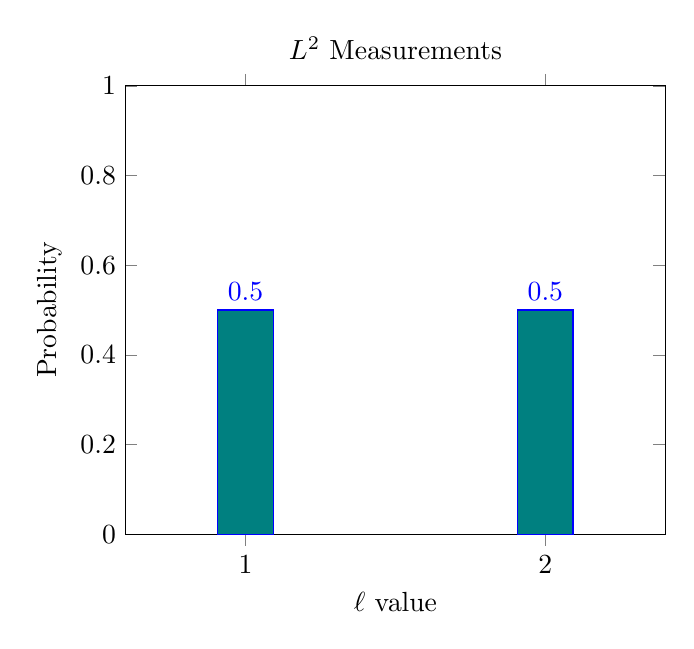
\begin{tikzpicture}
  \begin{axis}[
    ybar,
    bar width=20pt,
    enlarge x limits=0.4,
    ymin=0, ymax=1,
    ylabel={Probability},
    xtick=data,
    nodes near coords,
    xlabel = $\ell $ value,
    title = $L^2$ Measurements
  ]
    % <— Replace the numbers 0.3 and 0.7 with your own probabilities
    \addplot+[fill=teal] coordinates {
      (1, 0.5)
      (2, 0.5)
    };
  \end{axis}
\end{tikzpicture}

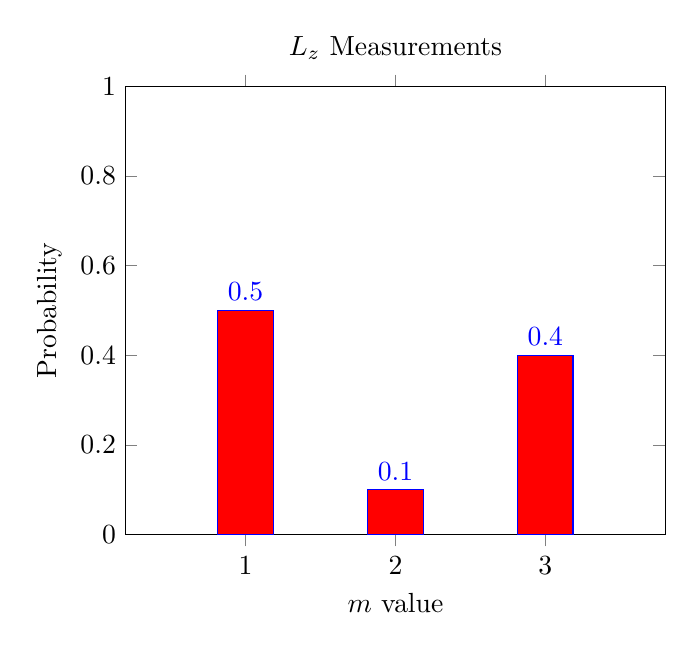
\begin{tikzpicture}
  \begin{axis}[
    ybar,
    bar width=20pt,
    enlarge x limits=0.4,
    ymin=0, ymax=1,
    ylabel={Probability},
    xtick=data,
    nodes near coords,
    xlabel = $m$ value,
    title = $L_z$ Measurements
  ]
    % <— Replace the numbers 0.3 and 0.7 with your own probabilities
    \addplot+[fill=red] coordinates {
      (1, 0.5)
      (2, 0.1)
      (3,0.4)
    };
  \end{axis}
\end{tikzpicture}
\end{center}
		
\end{enumerate}

\end{document}
